\chapter{Приложения}
\label{ch:appendix}

Схема установки для исследования плазмы газового разряда в неоне представлена на рис.~\ref{fig:ht}. 
Стеклянная газоразрядная трубка имеет холодный (ненагреваемый) полый катод, три анода и геттерный узел — стеклянный баллон, 
на внутреннюю поверхность которого напылён газопоглощающий плёнка (геттер). Трубка наполнена изотопом неона $^{22}$Ne при давлении 2 мм рт. ст. 
Катод и один из анодов (I или II) с помощью переключателя П$_1$ подключаются через балластный резистор $R_b \sim 450$ кОм 
к регулируемому высоковольтному источнику питания (ВИП) с выходным напряжением до 5 кВ.

\begin{figure}[ht]
    \centering
    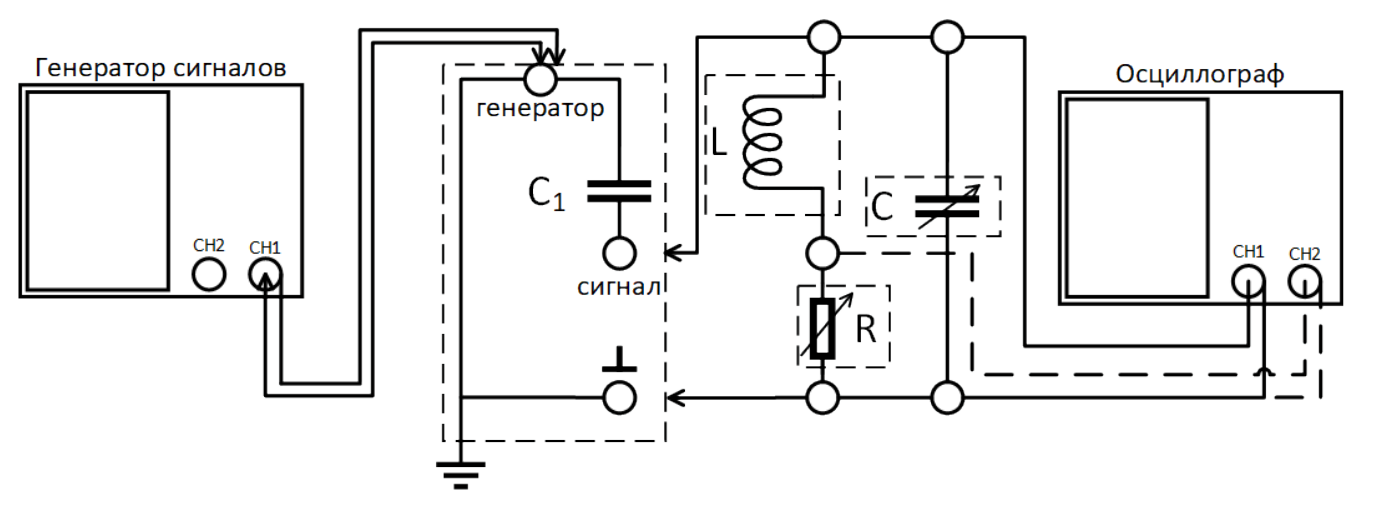
\includegraphics[width=0.8\linewidth]{./img/Установка.png}
    \caption{Схема установки}
    \label{fig:ht}
\end{figure}

При подключении к ВИП анода-I между ним и катодом возникает газовый разряд. 
Ток разряда измеряется миллиамперметром $A_1$, а падение напряжения на разрядной трубке — цифровым вольтметром $V_1$ (мультиметр GDM), 
подключённым к трубке через высокоомный (25 МОм) делитель напряжения с коэффициентом $(R_1 + R_2)/R_2 = 10$.

При подключении к ВИП анода-II разряд возникает в пространстве между катодом и анодом-II, 
где находится двойной зонд, используемый для диагностики плазмы положительного столба.

Зонды изготовлены из молибденовой проволоки диаметром $d = 0{,}2$ мм и имеют длину $l = 5{,}2$ мм. 
Они подключены к источнику питания GPS через потенциометр $R$. Переключатель П$_2$ позволяет изменять полярность напряжения на зондах. 
Величина напряжения на зондах изменяется с помощью дискретного переключателя «V» выходного напряжения источника питания и потенциометра $R$, 
а измеряется цифровым вольтметром $V_2$ (GDM). Для измерения зондового тока используется мультиметр $A_2$ (GDM). Анод-III в нашей работе не используется.